 \documentclass[11pt]{article} 
\usepackage[english]{babel}
\usepackage[utf8]{inputenc}
\usepackage[margin=0.5in]{geometry}
\usepackage{amsmath}
\usepackage{amsthm}
\usepackage{amsfonts}
\usepackage{amssymb}
\usepackage[usenames,dvipsnames]{xcolor}
\usepackage{graphicx}
\usepackage[siunitx]{circuitikz}
\usepackage{tikz}
\usepackage{tkz-berge}
\usetikzlibrary{positioning, automata, backgrounds}
\usepackage[colorinlistoftodos, color=orange!50]{todonotes}
\usepackage{hyperref}
\usepackage[numbers, square]{natbib}
\usepackage{fancybox}
\usepackage{epsfig}
\usepackage{soul}
\usepackage[framemethod=tikz]{mdframed}
\usepackage[shortlabels]{enumitem}
\usepackage[version=4]{mhchem}
\usepackage{multicol}
\usepackage{forest}
\usepackage{mathtools}
\usepackage{comment}
\usepackage{enumitem}
\usepackage[utf8]{inputenc}
\usepackage{listings}
\usepackage{color}
\usepackage[numbers]{natbib}
\usepackage{subfiles}
\usepackage{tkz-berge}
\usepackage{algorithm}
\usepackage[noend]{algpseudocode}


\newtheorem{prop}{Proposition}[section]
\newtheorem{thm}{Theorem}[section]
\newtheorem{lemma}{Lemma}[section]
\newtheorem{cor}{Corollary}[prop]

\theoremstyle{definition}
\newtheorem{definition}{Definition}

\theoremstyle{definition}
\newtheorem{required}{Problem}

\theoremstyle{definition}
\newtheorem{ex}{Example}

\newcommand{\interval}[4]{\draw (#2, #1) -- (#3, #1); % Usage: \interval{height}{start}{end}{label}
\draw (#2, #1-0.11) -- (#2, #1+0.11); % draw left whisker
\draw (#3, #1-0.11) -- (#3, #1+0.11); % draw right whisker
\node[] at (#2-0.25, #1) {#4};
}


\setlength{\marginparwidth}{3.4cm}
%#########################################################

%To use symbols for footnotes
\renewcommand*{\thefootnote}{\fnsymbol{footnote}}
%To change footnotes back to numbers uncomment the following line
%\renewcommand*{\thefootnote}{\arabic{footnote}}

% Enable this command to adjust line spacing for inline math equations.
% \everymath{\displaystyle}

% _______ _____ _______ _      ______ 
%|__   __|_   _|__   __| |    |  ____|
%   | |    | |    | |  | |    | |__   
%   | |    | |    | |  | |    |  __|  
%   | |   _| |_   | |  | |____| |____ 
%   |_|  |_____|  |_|  |______|______|
%%%%%%%%%%%%%%%%%%%%%%%%%%%%%%%%%%%%%%%

\title{
\normalfont \normalsize 
\textsc{CSCI 3104 Spring 2022 \\ 
Instructors: Profs. Chen and Layer} \\
[10pt] 
\rule{\linewidth}{0.5pt} \\[6pt] 
\huge Problem Set 7\\
\rule{\linewidth}{2pt}  \\[10pt]
}
%\author{Your Name}
\date{}

\begin{document}
\definecolor {processblue}{cmyk}{0.96,0,0,0}
\maketitle


%%%%%%%%%%%%%%%%%%%%%%%%%
%%%%%%%%%%%%%%%%%%%%%%%%%%
%%%%%%%%%%FILL IN YOUR NAME%%%%%%%
%%%%%%%%%%AND STUDENT ID%%%%%%%%
%%%%%%%%%%%%%%%%%%%%%%%%%%
\noindent
Due Date \dotfill March 15 \\
Name \dotfill \textbf{Your Name} \\
Student ID \dotfill \textbf{Your Student ID} \\
Collaborators \dotfill \textbf{List Your Collaborators Here}

\tableofcontents

\section{Instructions}
{\small
 \begin{itemize}
	\item The solutions \textbf{must be typed}, using proper mathematical notation. We cannot accept hand-written solutions. \href{http://ece.uprm.edu/~caceros/latex/introduction.pdf}{Here's a short intro to \LaTeX.}
	\item You should submit your work through the \textbf{class Canvas page} only. Please submit one PDF file, compiled using this \LaTeX \ template.
	\item You may not need a full page for your solutions; pagebreaks are there to help Gradescope automatically find where each problem is. Even if you do not attempt every problem, please submit this document with no fewer pages than the blank template (or Gradescope has issues with it).

	\item You are welcome and encouraged to collaborate with your classmates, as well as consult outside resources. You must \textbf{cite your sources in this document.} \textbf{Copying from any source is an Honor Code violation. Furthermore, all submissions must be in your own words and reflect your understanding of the material.} If there is any confusion about this policy, it is your responsibility to clarify before the due date. 

	\item Posting to \textbf{any} service including, but not limited to Chegg, Reddit, StackExchange, etc., for help on an assignment is a violation of the Honor Code.

\end{itemize}}


\newpage
\section{Standard 19 - Dynamic Programming: Identify the Precise Subproblems}

\noindent The goal of this standard is to practice identifying the recursive structure. To be clear, you are \textbf{not} being asked for a precise mathematical recurrence. Rather, you are being asked to clearly and precisely identify the cases to consider. Identifying the cases can sometimes provide enough information to design a dynamic programming solution.

\subsection{Problem \ref{DP1}}
\begin{required} \label{DP1}
Consider the \textsf{Stair Climbing} problem, defined as follows.
\begin{itemize}
\item \textsf{Instance:} Suppose we have $n$ stairs, labeled $s_{1}, \ldots, s_{n}$. Associated with each stair $s_{k}$ is a number $a_{k} \geq 1$. At stair $s_{k}$, we may jump forward $i$ stairs, where $i \in \{ 1, 2, \ldots, a_{k}\}$. You start on $s_{1}$.

\item \textsf{Solution:} The number of ways to to reach $s_{n}$ from $s_{1}$.
\end{itemize}

\noindent \\ \textbf{Your job} is to clearly identify the recursive structure. That is, suppose we are solving the subproblem at stair $s_{k}$. What precise sub-problems do we need to consider?
\end{required}

\begin{proof}[Answer]
%Your answer
\end{proof}



\newpage
\subsection{Problem \ref{DP2}}
\begin{required} \label{DP2}
Fix $n \in \mathbb{N}$. The \textit{Trust Game} on $n$ rounds is a two-player dynamic game. Here, Player I starts with \$100. The game proceeds as follows.
\begin{itemize}
\item \textbf{Round 1:} Player I takes a fraction of the \$100 (which could be nothing) to give to Player II. The money Player I gives to Player II is multiplied by 1.5 before Player II receives it. Player I keeps the remainder. (So for example, if Player I gives \$20 to Player II, then Player II receives \$30 and Player I is left with \$80).

\item \textbf{Round 2:} Player II can choose a fraction of the money they received to offer to Player I. The money offered to Player I increases by a multiple of $1.5$  before Player I receives it. Player II keeps the remainder.
\end{itemize}

\noindent \\ More generally, at round $i$, the Player at the current round (Player I if $i$ is odd, and Player II if $i$ is even) takes a fraction of the money in the current pile to send to the other Player and keeps the rest. That money increases by a factor of $1.5$ before the other player receives it. The game terminates if the current player does not send any money to the other player, or if round $n$ is reached. At round $n$, the money in the pile is split evenly between the two players. \\

\noindent Each individual player wishes to maximize the total amount of money they receive. \\

\noindent \textbf{Your job} is to clearly identify the recursive structure. That is, at round $i$, what precise sub-problems does the current player need to consider? [\textbf{Hint:} Do we have a smaller instance of the Trust Game after each round?]
\end{required}

\begin{proof}[Answer]
%Your answer
\end{proof}




\newpage
\section{Standard 20- Dynamic Programming: Write Down Recurrences}

\subsection{Problem \ref{DP3}}

\begin{required} \label{DP3}
Suppose we have an $m$-letter alphabet $\Sigma = \{0, 1, \ldots, m-1\}$. Let $W_{n}$ be the set of strings $\omega \in \Sigma^{n}$ such that $\omega$ does not have $00$ as a substring. Let $f_{n} := |W_{n}|$. Write down an explicit recurrence for $f_{n}$, including the base cases. Clearly justify each recursive term.
\end{required}

\begin{proof}[Answer]
%Your answer here.
\end{proof}

%You may find the following commented code helpful in rendering a recurrence
\begin{comment}
\begin{align*}
f_{n} &= \begin{cases} \text{Case1} & : \text{Condition1}, \\ 
\text{Case2} & : \text{Condition2}. 
\end{cases}
\end{align*}
\end{comment}




\newpage
\subsection{Problem \ref{DP4}}

\begin{required} \label{DP4}
Suppose we have the alphabet $\Sigma = \{x, y\}$. For $n \geq 0$, let $W_{n}$ be the set of strings $\omega \in \{x, y\}^{n}$ where $\omega$ contains $yyy$ as a substring. Let $f_{n} := |W_{n}|$. Write down an explicit recurrence for $f_{n}$, including the base cases. Clearly justify each recursive term.
\end{required}

\begin{proof}[Answer]
%Your answer here.
\end{proof}




\newpage
\section{Standard 21- Dynamic Programming: Using Recurrences to Solve}

\subsection{Problem \ref{Recurrence1}}
\begin{required} \label{Recurrence1}
Given the following directed acyclic graph. Use dynamic programming to fill in a \textbf{one-dimensional} lookup table that counts number of paths from each node $j$ to 14, for $j \geq 1$. Note that a single vertex is considered a path of length $0$. \textbf{Fill in the lookup table for all vertices 1-14; and in addition, clearly show work for vertices 9-14}.

        % ----- FIGURE -----
        \begin{figure}[h!]
        \begin{center}
        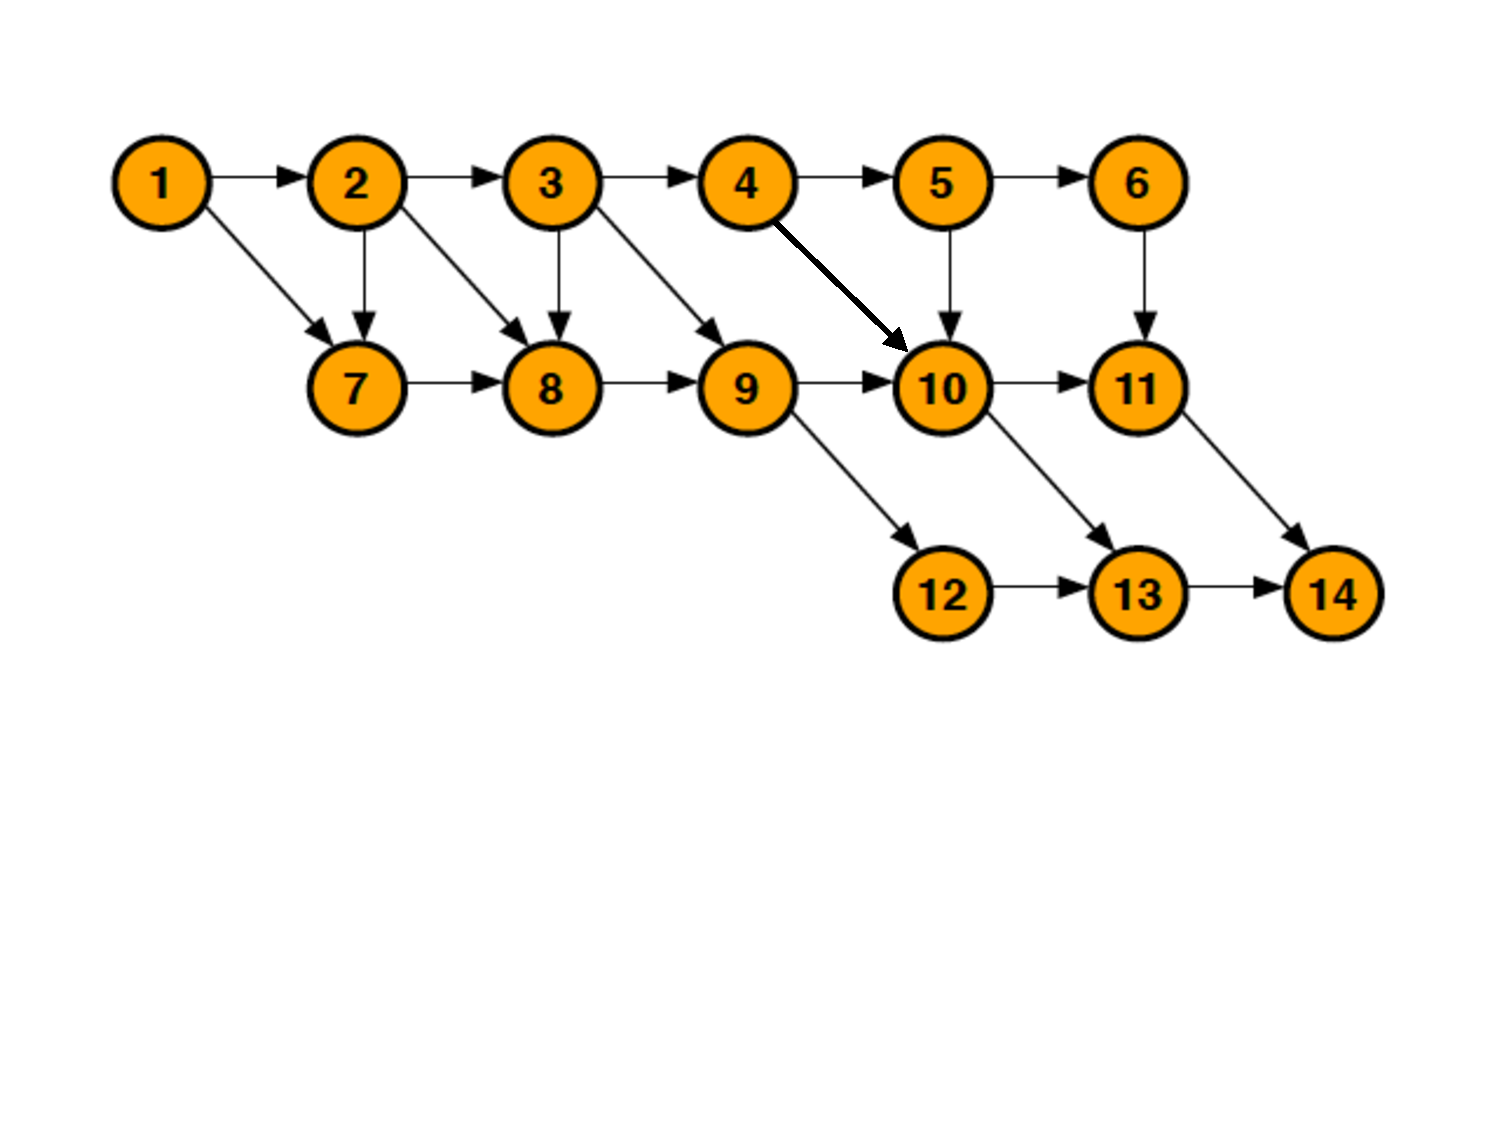
\includegraphics[scale=0.45]{dag_ps10.pdf} 
        \end{center}
        \end{figure}
        % ----------

\end{required}


\begin{proof}[Answer]
%Your answer
\end{proof}




\newpage
\subsection{Problem \ref{Recurrence2}}
\begin{required} \label{Recurrence2}
Consider the following input for the Knapsack problem with a capacity $W=12$:\\

 \begin{tabular}{r|c|c|c|c|c|c}
        item $i$  & 1  & 2 &3 &4 &5 &6 \\
                \hline
        value $v_i$ &2 & 7& 18&23 &29 &35 \\
          \hline
        weight $w_i$ & 1 & 2  & 5& 6& 7& 9\\
                 \end{tabular}

\vspace{1mm}
\noindent \\ 
Fill in a lookup table, similar to the example on page 12 of course notes for week 9 (see Week 9 under ``Modules" of the course canvas). In addition, clearly explain how you obtain the maximum values/profits $OPT(6, w)$, $w=7,~8,~9,~10,~11,~12$.

\end{required}

\begin{proof}[Answer]
%Your answer here
\end{proof}

\end{document} % NOTHING AFTER THIS LINE IS PART OF THE DOCUMENT



